% ****** Start of file apssamp.tex ******
%
%   This file is part of the APS files in the REVTeX 4 distribution.
%   Version 4.0 of REVTeX, August 2001
%
%   Copyright (c) 2001 The American Physical Society.
%
%   See the REVTeX 4 README file for restrictions and more information.
%
% TeX'ing this file requires that you have AMS-LaTeX 2.0 installed
% as well as the rest of the prerequisites for REVTeX 4.0
%
% See the REVTeX 4 README file
% It also requires running BibTeX. The commands are as follows:
%
%  1)  latex apssamp.tex
%  2)  bibtex apssamp
%  3)  latex apssamp.tex
%  4)  latex apssamp.tex
%
\documentclass[prb,aps,preprintnumbers,amsmath,amssymb]{revtex4}
%\documentclass[preprint,showpacs,preprintnumbers,amsmath,amssymb]{revtex4}

% Some other (several out of many) possibilities
%\documentclass[preprint,aps]{revtex4}
%\documentclass[preprint,aps,draft]{revtex4}
%\documentclass[prb,twocolumn,showpacs,preprintnumbers,amsmath,amssymb]{revtex4}% Physical Review B

\usepackage{graphicx}% Include figure files
\usepackage{dcolumn}% Align table columns on decimal point
\usepackage{bm}% bold math
\usepackage[utf8]{inputenc}
\usepackage{url}
\newcommand{\nextitem}{\par\hspace*{\labelsep}\textbullet\hspace*{\labelsep}}
%\nofiles

\begin{document}

\title{Preinforme 3 - Amplificadores Operacionales}% Force line breaks with \\

\author{Alejandro Hernández A.}%
 \email{a.hernandez105@uniandes.edu.co}
\author{Jesús D. Prada G.}%
 \email{jd.prada1460@uniandes.edu.co}
\affiliation{%
Departamento de Física\\ Universidad de los Andes, Bogotá, Colombia.\\
}%

\date{16 de septiembre de 2015}% It is always \today, today,
             %  but any date may be explicitly specified

\begin{abstract}
En esta práctica de laboratorio se pretende aprender el funcionamiento experimental de amplificadores operacionales y mediante el uso de los mismos se pretende armar filtros activos y pasivos.\\

\noindent \textbf{Conceptos clave:} Amplificadores operacionales, filtros activos, filtros pasivos, ganancia.
\end{abstract}
                             
\maketitle

\section{Filtros activos y pasivos}
Como se ha mencionado en preinformes anteriores, un filtro es un sistema que permite el paso de señales eléctricas en un rango de
frecuencias determinadas e impide el paso del resto.\\

Un \textbf{filtro activo} se caracteriza por el uso de componentes activos. Dichos componentes se caracterizan por controlar el flujo de corriente en los circuitos o por realizar ganancias. Dichos elementos se enuncian a continuación \footnote{Información consultada en http://es.slideshare.net/electronicosdigitales/componentes-activos\\}.

\begin{itemize}
	\item \textbf{Amplificador operacional}: Como se puede apreciar en la figura \ref{fig: amplificador}, los amplificadores operacionales son dispositivos electrónicos con dos entradas y una salida, en la última de las cuales el potencial medido es la diferencia de potencial entre las dos entradas multiplicada por una constante $G$ que representa la ganancia de l sistema.
	
	\begin{figure}[h!]
		\centering
		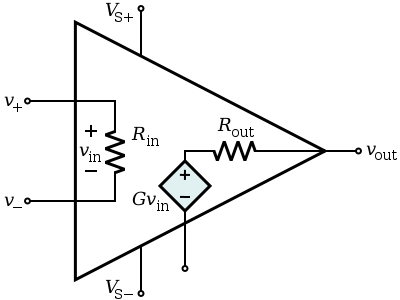
\includegraphics[width=0.5\textwidth]{amplificador}
		\caption{Amplificador operacional.}
		\label{fig: amplificador}
	\end{figure}
	
	\item \textbf{Diodos}: Típicamente utilizados para la rectificación y regulación de señales. 
	
	\item \textbf{Baterías}: Usadas para la generación de energía eléctrica.
	
	\item \textbf{Compuertas lógicas}: Empleadas para controlar el paso de la corriente eléctrica en un circuito de acuerdo con la función booleana asociada.
	
	\item \textbf{Transistor}: Usados para la amplificación o conmutación de señales.
\end{itemize}

Por su parte, los \textbf{filtros pasivos} se caracteriazan por usar componentes pasivos, en los cuales la potencia eléctrica absorbida es transformada en calor y que no son capaces de controlar el flujo de la corriente eléctrica. Estos componentes son los tres componentes típicos de cualquier circuito eléctrico, a saber\footnote{Información consultada en http://www.ecured.cu/index.php/Componentes\_electr\%C3\%B3nicos\_pasivos\\}: \\\\

\begin{itemize}
	\item \textbf{Resistencias}: Permiten controlar la corriente que pasa a través de un circuito.
		
	\item \textbf{Condensadores}: Sirven para almacenar energía en forma de carga eléctrica. 
	
	\item \textbf{Inductancias}: Se oponen al cambio del flujo de campo magnético a través de las mismas.
\end{itemize}

\begin{figure}
\centering
\begin{minipage}{.33\textwidth}
  \centering
  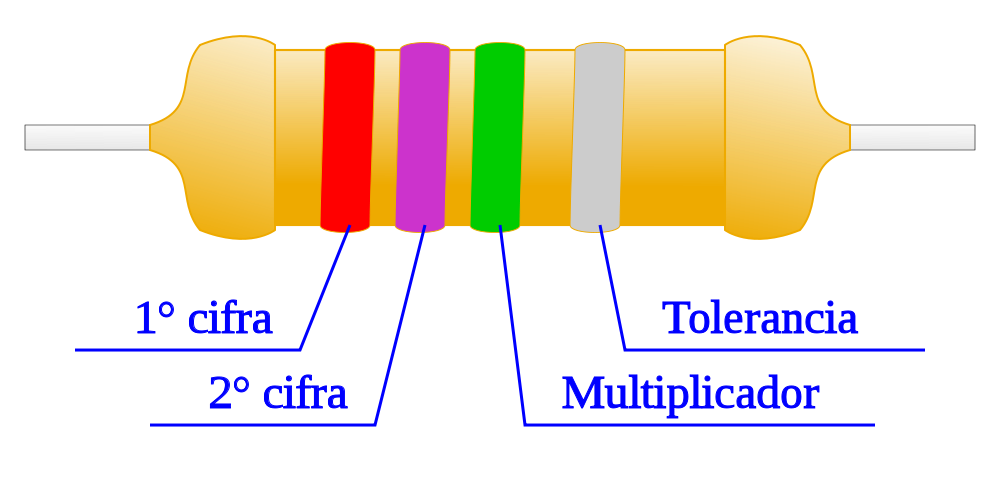
\includegraphics[width=.7\textwidth,height=0.15\textheight]{resistencia}
  \caption{Resistencia}
  \label{fig: resistencia}
\end{minipage}%
\begin{minipage}{.33\textwidth}
  \centering
  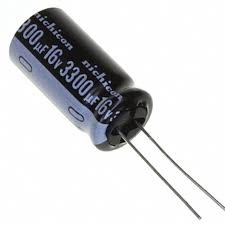
\includegraphics[width=.7\textwidth,height=0.15\textheight]{condensador}
  \caption{Condensador}
  \label{fig: condensador}
\end{minipage}
\begin{minipage}{.33\textwidth}
  \centering
  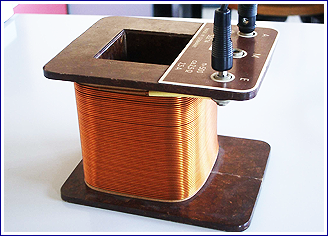
\includegraphics[width=.7\textwidth,height=0.15\textheight]{inductancia}
  \caption{Inductancia}
  \label{fig: inductancia}
\end{minipage}
\label{fig: pasivos}
\end{figure}

Las ventajas y desventajas de usar un filtro u otro se muestran a continuación \footnote{La información presentada se consultó en http://www.mty.itesm.mx/etie/deptos/ie/profesores/jgomez/eap/filtros.pdf\\}.\\

\textbf{Ventajas de los filtros activos}

\begin{itemize}
	\item Pueden ser usados sin inductancias, que son dispositivos electrónicos difíciles de conseguir, además de ser muy voluminosos para frecuencias bajas.
	
	\item Facilitan el montaje de filtros complejos mediante el ensamble de múltiples filtros simples.
	
	\item Proporcionan un gran ganancia, es decir, son buenos amplificadores de la señal de entrada, lo cual es especialmente útil.
	
	\item Se adaptan muy bien a las impedancias.
\end{itemize}

\textbf{Desventajas de los filtros activos}

\begin{itemize}
	\item Requieren de una fuente de alimentación externa para poder funcionar.
	
	\item Presentan una respuesta en freucuencia altamente limitada por la capacidad de los amplificadores operacionales usados.
	
	\item Es imposible implementar filtros activos en sistemas de media o alta potencia.
\end{itemize}

\textbf{Ventajas de los filtros pasivos}

\begin{itemize}
	\item Son económicos dado que sus componentes (salvo las inductancias) son de uso muy frecuente para el montaje de circuitos eléctricos básicos.
	
	\item Son fáciles de implementar.
	
	\item Su funcionamiento muestra una respuesta aproximada a la función ideal.
	
	\item Pueden ser usados en circuitos de altas frecuencias o altas potencias.
\end{itemize}

\textbf{Desventajas de los filtros pasivos}

\begin{itemize}
	\item La respuesta en frecuencia está limitada al valor de los componentes pasivos usados.
	
	\item Las inductancias no son fáciles de conseguir y su valor económico se incrementa para altas frecuencias.
\end{itemize}

Con respecto a las aplicaciones de dichos filtros, cabe mencionar que los filtros activos son frecuentemente usados en istrumentación y telecomunicaciones. En cuanto a la instrumentación, los dispositivos de bioelectrónica o electromedicina típicamente incluyen este tipo de filtros puesto que necesitan trabajar con señales de bajas frecuencias. \\

Los filtros tanto activos como pasivos también se usan para aumentar o atenuar frecuencias en circuitos de audio, generadores electrónicos de música, instrumentos sísmicos y circuitos de comunicaciones. Además, en ámbitos experimentales o de laboatorio, son utilizados para estudiar señales de ondas cerebrales y vibraciones mecánicas.\\

<<<<<<< HEAD
\section{Tipos de filtros ativos}

=======
\section{Filtros pasa bajas}
Un filtro activo pasa bajas es un filtro que amplifica las señales con frecuencia baja, mientras que reduce las señales con frecuencias altas. Un montaje de circuito pasa bajas activo se muestra en la siguiente figura.\\

\begin{figure}[h!]
  \centering
  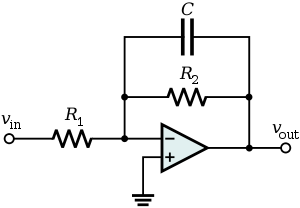
\includegraphics[width=.5\textwidth]{low}
  \caption{Filtro activo pasa bajas}
  \label{fig:pasabajas}
\end{figure}

Cualitativamente lo que está pasando en el circuito de la anterior figura es que a frecuencias bajas, con periodos mucho más altos que el tiempo de carga característico del condensador, dicho elemento se alcanza a cargar considerablemente. Cuando el capacitor se carga funciona aproximadamente como un interruptor abierto, dejando pasar corriente por la resistencia $R_2$. En este caso, tendríamos una ganancia dada por $\frac{R_2}{R_1}$, como un amplificador normal. En el caso de frecuencias altas, con periodos mucho más bajos que el tiempo característico del condensador, dicho elemento no se alcanza a cargar. Dado que un capacitor cargado funciona aproximadamente como un corto circuito, la corriente tendería a fluir por allí con resistencia nula, en vez  de pasar por $R_2$. En este caso, tendríamos un amplificador normal con $R'_2 = 0$, por lo que la ganancia estaría dada por $0$, es decir, no deja pasar señales con frecuencias altas.\\

Cabe resaltar que hay una transición suave entre frecuencias altas y bajas que no describimos aquí, pero que podemos asumir. En un filtro ideal, esta transición sería empinada como una función Heaviside.\\

Con esta explicación podemos concluir que en este circuito las resistencias $R_1$ y $R_2$ actúan como amplificadoras definiendo la ganancia y además el tiempo característico del capacitor ($\tau = R_2C$), mientras que el capacitor es la parte funcional del filtro que deja pasar señales con frecuencia baja ($\omega < \omega_C = \frac{1}{R_2C}$).\\

\section{Filtros pasa altas}
Un filtro pasa altas, análogamente a un cricuito pasa bajas, amplifica las señales de frecuencias altas y reduce las señales de frecuencias bajas. En la siguiente figura se muestra un filtro activo pasa altas.\\

\begin{figure}[h!]
  \centering
  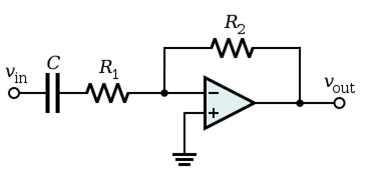
\includegraphics[width=.5\textwidth]{high}
  \caption{Filtro activo pasa altas}
  \label{fig: pasaaltas}
\end{figure}

Cualitativamente lo que pasa en este circuito es lo siguiente: A frecuencias altas, con periodos mucho más bajos que el tiempo característico del condensador, el capacitor al lado de la resistencia $R_1$ no se alcanza a cargar mucho, por lo que se podría tomar como un corto circuito. En este caso lo que se tiene es un amplificador normal con ganancia dada por $\frac{R_2}{R_1}$. Por otra parte, a frecuencias bajas, con periodos mucho más altos que el tiempo característico del condensador, el capacitor se alcanza a cargar, comportándose así como un interruptor abierto. En este caso, dado que "abrimos" el circuito, el voltaje de salida será nulo (o casi nulo) y la ganancia será $0$.\\


En este caso, podemos afirmar lo mismo que afirmamos anteriormente. Las resistencias actúan como amplificadoras definiendo la ganancia y además el tiempo característico del capacitor ($\tau = R_1C$), mientras que el capacitor es la parte funcional del filtro, el cual deja pasar señales con frecuencias altas ($\omega > \omega_C = \frac{1}{R_1C}$).\\

\section{Filtros pasa bandas}
Un filtro pasabandas, como su nombre lo dice, amplifica señales con frecuencia en una banda. En otras palabras, este filtro amplifica todas las señales con frecuencia mayor a cierto valor límite inferior, y menor a cierto valor límite superior. Un filtro pasa bandas activo se muestra en la siguiente figura.\\

\begin{figure}[h!]
  \centering
  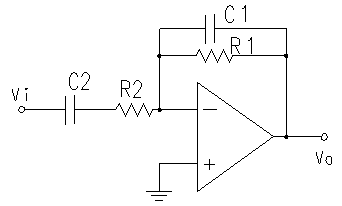
\includegraphics[width=.5\textwidth]{band}
  \caption{Filtro activo pasa bandas}
  \label{fig: pasabandas}
\end{figure}

En este claramente se puede observar que su parte izquierda es análoga a un circuito pasa altas, mientras su parte derecha es análoga al circuito pasa bajas. Claramente consiste de un amplificador pasa altas acoplado a un amplificador pasa bajas. En este caso no es necesario explicar como funciona, dado que el efecto es la conjunción de los dos efectos pasa bajas y altas, que ya de por sí son muy análogos entre ellos.\\

En este caso claramente podemos identificar las resistencias como amplificadoras que definen la ganancia y los tiempos característicos límites de los capacitores ($\tau_1 = R_1C_1$, $\tau_2 = R_2C_2$), los cuales serán la parte funcional del filtro al dejar pasar las señales con frecuencias en la banda. El capacitor $C_2$ deja pasar solo señales con altas frecuencias ($\omega > \frac{1}{\tau_2}$), mientras el capacitor $C_1$ deja pasar solo señales con bajas frecuencias ($\omega < \frac{1}{\tau_1}$). En este sentido, ambos capacitores actuando en conjunto nos determinan la banda de frecuencias que pueden pasar amplificadas ($\frac{1}{\tau_1} > \omega > \frac{1}{\tau_2}$). Claramente, la ganancia de amplificación está dada por $\frac{R_1}{R_2}$. \\

Claramente se requiere $\tau_2 > \tau_1$, ya que de otra manera, la desigualdad definiría una banda vacía.\\

\section{Planeación}
Para este laboratorio planeamos hacer al menos los filtros pasa altas y pasa bajas. Para esto utilizaremos un amplificador operacional de referencia LM358P. A este amplificador lo alimentaremos con una fuente de voltaje DC entre 10 y 12 voltios, al igual que hicimos en el anterior laboratorio.\\

Además de esto, usaremos resistencias que ya sabemos que van de la mano con este amplificador, las cuales son de $15k\Omega$ y de $1.5k\Omega$. En principio crearemos el filtro con ganancia 0.1 o 1, dado que ya vimos que usar ganancia 10 puede superar los límites aceptados por el osciloscopio. Si necesitamos una ganancia diferente podemos jugar con estas resistencias en serie para crear números decimales, después de todo, son las más numerosas en nuestro kit.\\

En cuanto a los capacitores usaremos capacitores 334 ($330n F$). Si queremos hacer el circuito pasabandas podemos jugar con estos capacitores en paralelo para no confundirse con los límites de la banda. En general, estos capacitores con las resistencias mencionadas producen pares RC con tiempos característicos de $\frac{1}{RC} \approx (200-2000) Hz$, lo cual es un rango aceptable según la ficha técnica del amplificador.\\

En cuanto al voltaje de entrada, será AC claramente, y procuraremos mantenerlo alrededor de los 5V, ya que, por experiencia, es un voltaje de entrada que va de la mano con el amplificador operacional a utilizar y las resistencias mencionadas. Si es el caso, podremos subirlo un poco por los efectos del capacitor que posiblemente atenue un poco la señal. El capacitor se comporta como circuito abierto o corto circuito en el límite $t\rightarrow\infty$, lo cual nunca sucede.\\
>>>>>>> 334dbc4630ecb3e3f41199bd2d7883d55b8fce00

\begin{thebibliography}{99}
\
\\
\bibitem{resistencia} La imagen de la resistencia se obtuvo en http://www.areatecnologia.com/electricidad/resistencia-electrica.html.\\

\bibitem{condensador} La imagen del condensador se obtuvo en http://logicadigitaltemario2.blogspot.com.co/2015/04/condensador.html.\\

\bibitem{inductancia} La imagen de la inductancia se obtuvo en http://www.electricaindustrialmaldonado.com/fabricacion-de-bobinas.\\


\end{thebibliography}

\end{document}
%
% ****** End of file apssamp.tex ******
